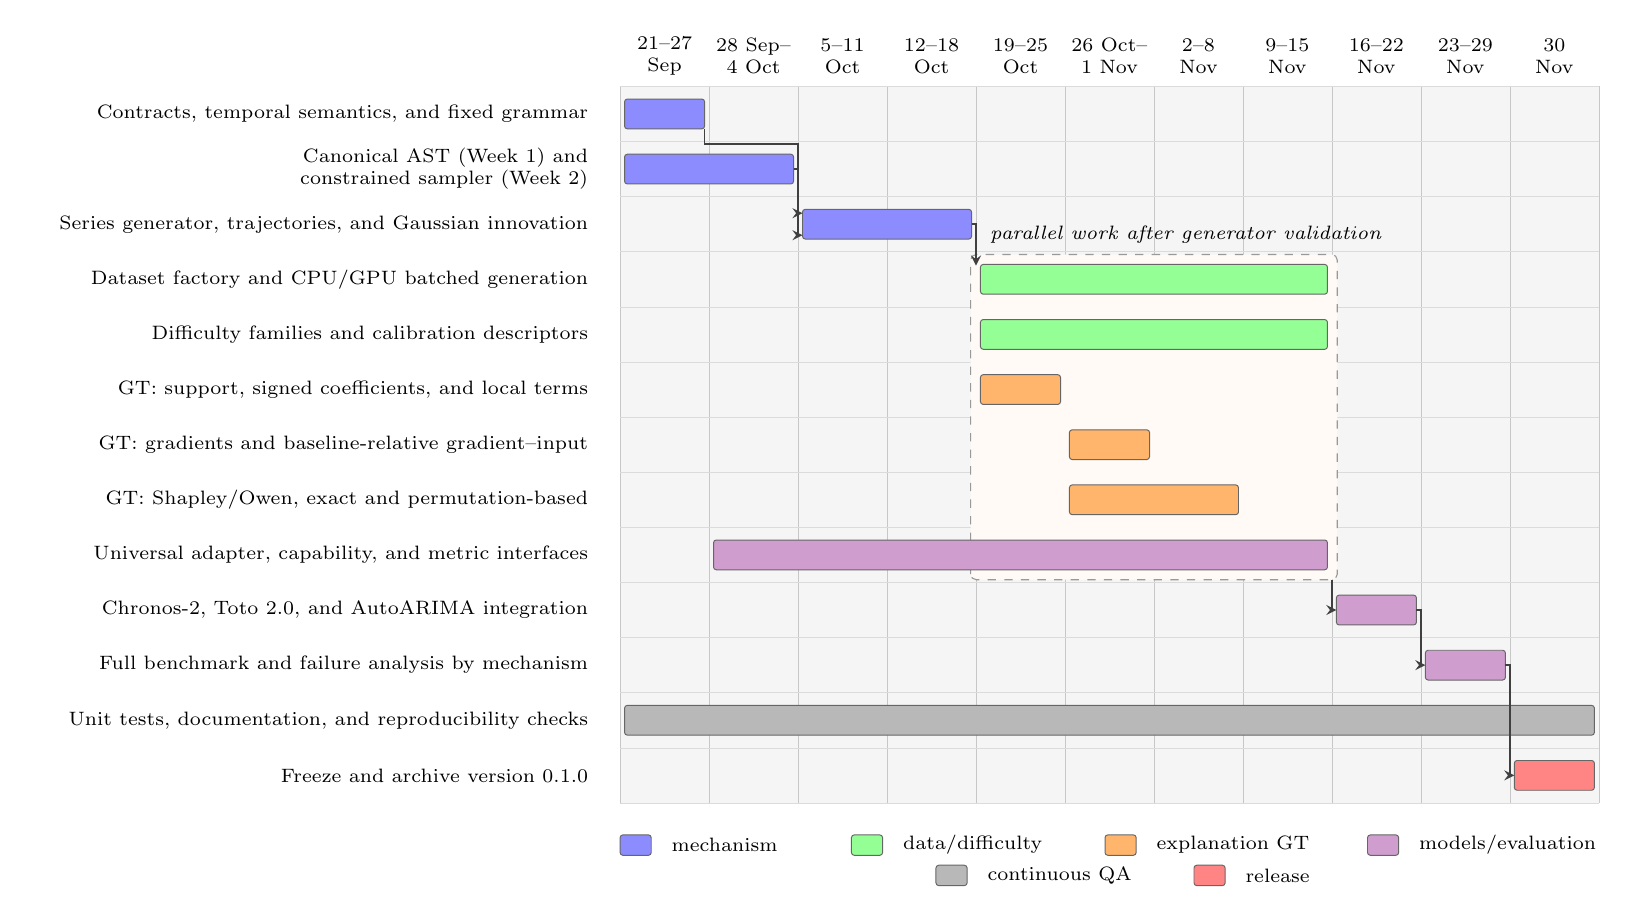
\begin{tikzpicture}[
    x=1.13cm,
    y=0.70cm,
    tasklabel/.style={font=\scriptsize,anchor=east,align=right,text width=7.0cm},
    bar/.style={draw=black!60,line width=0.35pt,rounded corners=1pt},
    dependency/.style={->,>=stealth,semithick,draw=black!75},
    legend/.style={font=\scriptsize,anchor=west}
]

% Timeline grid.
\fill[black!4] (0,-0.5) rectangle (11,12.5);
\foreach \x in {0,...,11} {
    \draw[black!22,line width=0.25pt] (\x,-0.5) -- (\x,12.5);
}
\foreach \y in {-0.5,0.5,...,12.5} {
    \draw[black!14,line width=0.2pt] (0,\y) -- (11,\y);
}

% Week headings.
\node[font=\scriptsize,align=center] at (0.5,13.05) {21--27\\Sep};
\node[font=\scriptsize,align=center] at (1.5,13.05) {28 Sep--\\4 Oct};
\node[font=\scriptsize,align=center] at (2.5,13.05) {5--11\\Oct};
\node[font=\scriptsize,align=center] at (3.5,13.05) {12--18\\Oct};
\node[font=\scriptsize,align=center] at (4.5,13.05) {19--25\\Oct};
\node[font=\scriptsize,align=center] at (5.5,13.05) {26 Oct--\\1 Nov};
\node[font=\scriptsize,align=center] at (6.5,13.05) {2--8\\Nov};
\node[font=\scriptsize,align=center] at (7.5,13.05) {9--15\\Nov};
\node[font=\scriptsize,align=center] at (8.5,13.05) {16--22\\Nov};
\node[font=\scriptsize,align=center] at (9.5,13.05) {23--29\\Nov};
\node[font=\scriptsize,align=center] at (10.5,13.05) {30\\Nov};

% Task labels.
\node[tasklabel] at (-0.25,12) {Contracts, temporal semantics, and fixed grammar};
\node[tasklabel] at (-0.25,11) {Canonical AST (Week 1) and constrained sampler (Week 2)};
\node[tasklabel] at (-0.25,10) {Series generator, trajectories, and Gaussian innovation};
\node[tasklabel] at (-0.25,9) {Dataset factory and CPU/GPU batched generation};
\node[tasklabel] at (-0.25,8) {Difficulty families and calibration descriptors};
\node[tasklabel] at (-0.25,7) {GT: support, signed coefficients, and local terms};
\node[tasklabel] at (-0.25,6) {GT: gradients and baseline-relative gradient--input};
\node[tasklabel] at (-0.25,5) {GT: Shapley/Owen, exact and permutation-based};
\node[tasklabel] at (-0.25,4) {Universal adapter, capability, and metric interfaces};
\node[tasklabel] at (-0.25,3) {Chronos-2, Toto 2.0, and AutoARIMA integration};
\node[tasklabel] at (-0.25,2) {Full benchmark and failure analysis by mechanism};
\node[tasklabel] at (-0.25,1) {Unit tests, documentation, and reproducibility checks};
\node[tasklabel] at (-0.25,0) {Freeze and archive version 0.1.0};

% Parallel work window after the first validated generator.
\filldraw[fill=orange!4,draw=black!40,dashed,rounded corners=2pt]
    (3.94,3.55) rectangle (8.06,9.45);
\node[font=\scriptsize\itshape,anchor=south west] at (4.05,9.48)
    {parallel work after generator validation};

% Core mechanism construction.
\filldraw[bar,fill=blue!45] (0.05,11.73) rectangle (0.95,12.27);
\filldraw[bar,fill=blue!45] (0.05,10.73) rectangle (1.95,11.27);
\filldraw[bar,fill=blue!45] (2.05,9.73) rectangle (3.95,10.27);

% Scalable generation and controlled difficulty.
\filldraw[bar,fill=green!42] (4.05,8.73) rectangle (7.95,9.27);
\filldraw[bar,fill=green!42] (4.05,7.73) rectangle (7.95,8.27);

% Explanation-ground-truth methods.
\filldraw[bar,fill=orange!58] (4.05,6.73) rectangle (4.95,7.27);
\filldraw[bar,fill=orange!58] (5.05,5.73) rectangle (5.95,6.27);
\filldraw[bar,fill=orange!58] (5.05,4.73) rectangle (6.95,5.27);

% Evaluation interface and model study.
\filldraw[bar,fill=violet!38] (1.05,3.73) rectangle (7.95,4.27);
\filldraw[bar,fill=violet!38] (8.05,2.73) rectangle (8.95,3.27);
\filldraw[bar,fill=violet!38] (9.05,1.73) rectangle (9.95,2.27);

% Continuous quality work and final milestone.
\filldraw[bar,fill=black!28] (0.05,0.73) rectangle (10.95,1.27);
\filldraw[bar,fill=red!48] (10.05,-0.27) rectangle (10.95,0.27);

% Hard dependency gates.
\draw[dependency] (0.95,11.73) -- (0.95,11.45) -- (2.00,11.45)
    -- (2.00,10.20) -- (2.05,10.20);
\draw[dependency] (1.95,11) -- (2.00,11) -- (2.00,9.80) -- (2.05,9.80);
\draw[dependency] (3.95,10) -- (4.00,10) -- (4.00,9.25);
\draw[dependency] (8.00,3.55) -- (8.00,3) -- (8.05,3);
\draw[dependency] (8.95,3) -- (9.00,3) |- (9.05,2);
\draw[dependency] (9.95,2) -- (10.00,2) -- (10.00,0) -- (10.05,0);

% Legend, split over two rows to remain readable after page scaling.
\filldraw[bar,fill=blue!45] (0,-1.45) rectangle (0.35,-1.08);
\node[legend] at (0.47,-1.265) {mechanism};
\filldraw[bar,fill=green!42] (2.60,-1.45) rectangle (2.95,-1.08);
\node[legend] at (3.07,-1.265) {data/difficulty};
\filldraw[bar,fill=orange!58] (5.45,-1.45) rectangle (5.80,-1.08);
\node[legend] at (5.92,-1.265) {explanation GT};
\filldraw[bar,fill=violet!38] (8.40,-1.45) rectangle (8.75,-1.08);
\node[legend] at (8.87,-1.265) {models/evaluation};

\filldraw[bar,fill=black!28] (3.55,-2.00) rectangle (3.90,-1.63);
\node[legend] at (4.02,-1.815) {continuous QA};
\filldraw[bar,fill=red!48] (6.45,-2.00) rectangle (6.80,-1.63);
\node[legend] at (6.92,-1.815) {release};

\end{tikzpicture}
